\chapter{相关研究现状分析}

本章节主要阐述数据立方计算的相关研究,分别从单机与分布式两个方面进行阐述。单机的算法主要包括 PipeSort 与 BUC。分布式的算法从两个方面进行阐述,一个是面向代数度量的 Naive 算法,另一个是面向整体性度量的 MR-Cube算法。

\section{单机数据立方的计算研究}

%数据立方的计算涉及到对原事实表数据进行扫描,对相应的 GroupBy 属性值执行聚合计算以及生成相应的立方数据等几个步骤。在数据立方计算的问题讨论中,如何尽可能地减少原事实表的数据扫描次数、降低 I/O 代价以及内存的开销,成为评价一个立方计算方法高效性的几个关键要点。

PipeSort \cite{agarwal1996computation} 与 BUC \cite{beyer1999bottom} 是两种经典且目前较为通用的数据立方计算方法。虽然这两种方法在提出时是基于单机实现的,但它们的计算思想对当前分布式数据立方计算有着非常重要的影响。分布式数据立方计算的实质是将数据划分到各个节点上进行并行计算,因此在单个节点上依然要使用单机的数据立方计算方法。

PipeSort 是自顶向下的计算,而 BUC 则是自底向上的计算方法。图 \ref{4_dimension_lattice}展示了一个 4 维数据立方的 lattice,其中 A,B,C,D 均为属性维度。在一个数据立方的 lattice 中,每一个节点代表一个region,箭头从父节点指向子节点。自顶向下的计算,就是在一个 lattice 中从父节点开始往下计算,而自底向上则相反。

\begin{figure}[!htb]
\centering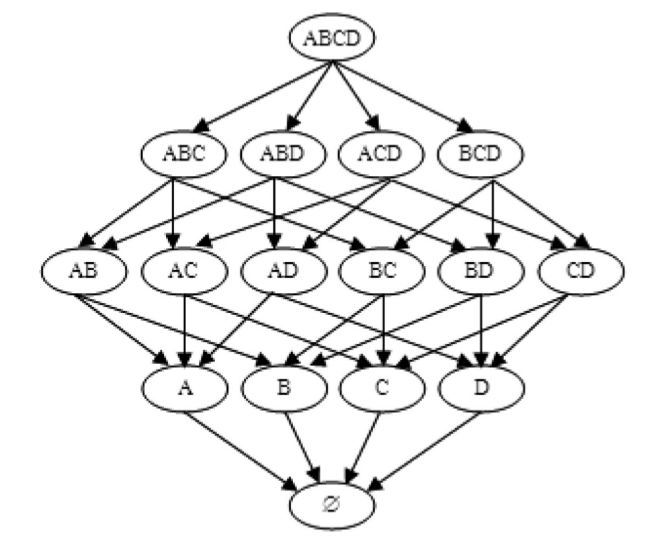
\includegraphics[width=3in]{picture/ch_current_research/4_dimension_lattice} 
\caption{4维数据立方的Lattice}\label{4_dimension_lattice} 
\end{figure} 

%\subsection{GBLP}

%Jim Gary 等人在提出数据立方概念的同时,还提出了一种计算数据立方的算法 —— GBLP \cite{gray1997data}。该算法的核心思想是自顶向下,为每个region选择其最小的父region(最小的region指该region内group数量最少的region)作为其计算的基础。对于一个 lattice,越往下,region内group的数量就会变得越少,因此相对于每个region都基于原始数据表进行计算,基于最小父region的计算能因为数据量的大规模减少而加快一个region的计算速度。但该方法只是把一个 lattice 修剪成一个树型结构,却没有提供一个特定的 lattice 遍历计划。另外当计算数据量很大无法完全存储于内存时,该方法没有提供一个有效的磁盘访问策略,这使得该方法的 I/O 代价会很高。

\subsection{PipeSort}

1996 年,Agarwal 等人针对 GBLP  \cite{gray1997data} 算法的缺陷,提出了第一个改进的数据立方计算方法 —— PipeSort\cite{agarwal1996computation} 。Pipe即Pipeline,流水线的意思。
PipeSort的核心思想是,在一个 lattice 中,假如一个region的维属性顺序是它其中一个父region的维属性顺序的前缀,则该region可以在其父region的基础上计算而无需额外的排序。若父region的属性数量较多,则可形成Pipeline(流水线)。

如图\ref{4_dimension_lattice} 所示的数据立方,假设每个region的维属性顺序就是图示的region名字从左到右的维顺序,例如对于region(ABC),维顺序指数据首先按照维属性 A 排序,若 A 相同的情况下再按照 B 排序,以此类推。region(AB) 的维顺序是region(ABC) 的前缀,但region(AC) 不是region(ABC) 的前缀。在这样的情况下,region(AB) 可从 region(ABC)计算获得,并且仅需要在内存中缓存一条元祖数据即可。因为数据按照维属性排序,具有相同AB值的数据必定排列在一起。同理,region(ABC) 可从 region(ABCD) 计算获得,于是形成了Pipeline(流水线) $ABCD\rightarrow ABC\rightarrow AB\rightarrow A$。因此对原数据和一些region进行多次排序,即可生成多条Pipeline。

PipeSort 采样估算每个region的大小,通过二分匹配的方法找出每个region需要从哪个父region计算获得。然后基于这个二分匹配的结果将一个 lattice 切割成多棵子树,称为 Pipeline (流水线),Pipeline 内只需对起始region的数据进行排序。对于每个 Pipeline,从起始region逐层往下计算,除起始region外,对于其他region,只需在内存中为其缓存一条元组,极大地节省了内存的使用率。但是,当数据立方的维度变得很高时,PipeSort 的排序代价会大大地增长。当数据比较稀疏时,排序的中间结果不能完全存储于内存中,还需进行外部排序,增加了 I/O 代价。图\ref{pipesort} 为 4 维数据立方使用 PipeSort 算法的计算过程。图(a)中的虚线表示从父region排序后得到子region的过程,实线表示流水线的计算过程。图(b)是最终需要计算的流水线,椭圆中的region表示需要重新排序。


\begin{figure}[!htb]
\centering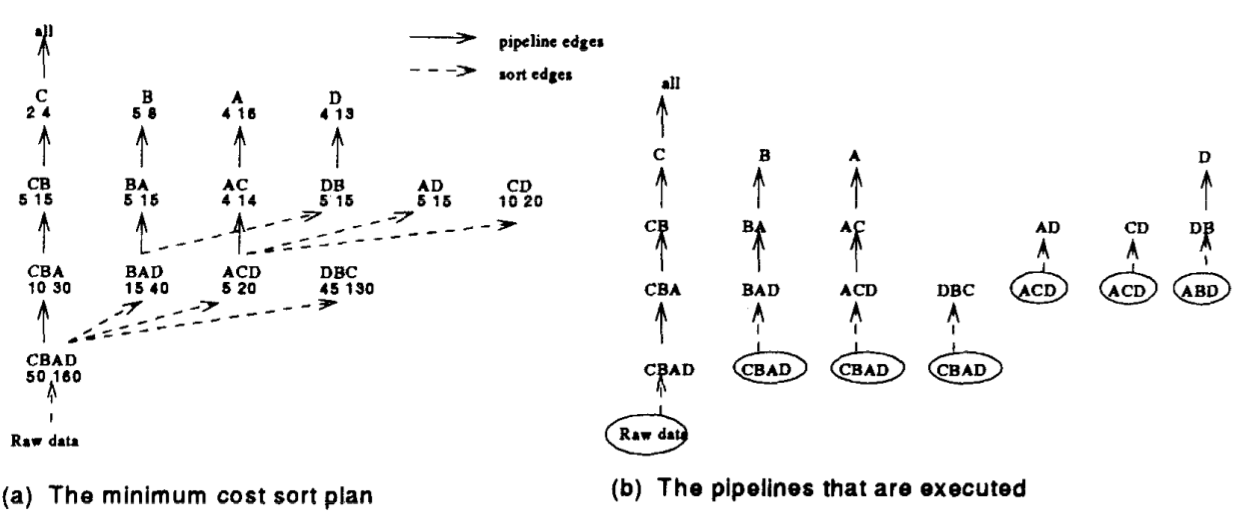
\includegraphics[width=5.5in]{picture/ch_current_research/pipesort} 
\caption{4维数据立方 PipeSort 计算过程}\label{pipesort} 
\end{figure} 

PipeSort 算法会将数据立方的计算分成多条 Pipeline 进行处理,正好与 MapReduce 中各个 reducer 并行处理多组数据类似,因此可将各个Pipeline的数据与计算分派给各个reducer,从而并行计算数据立方。并且MapReduce框架本身提供了对数据排序的功能,因此可以使用该功能对数据按照维度属性进行排序。同时,PiepSort 对数据只扫描一次即可计算Pipeline中的各个group,这个特性与MapReduce中reducer的迭代器有非常好的整合。因为reducer的迭代器仅能对数据进行一次扫描,若在reducer中要对数据进行多次扫描,需要将数据载入内存或者再次读取文件,加重了I/O操作。以上的这些原因这也正是 TSP-Cube 提出使用 PipeSort 的原因。

\subsection{BUC}

相对于PipeSort的自顶向下的数据立方计算方法,Beyer 等人在 1999 年提出的 BUC (Bottom Up Cube) 则是一种自底向上的算法。BUC 算法是针对冰山数据立方,即基于最少阈值的 GroupBy 计算而提出的,也即具有 HAVING 条件的 GroupBy,例如 HAVING COUNT(*) > 100 这样的条件限制。由于大部分的度量函数是具有单调性的,例如 COUNT(),若 Group(A=a0) 的结果是小于 100,那么 Group(A=a0, B=b0) 的结果必然是小于 100。正是这种单调性,加上有阈值限制,将数据立方的计算变成自底向上,则可以实现一定的剪枝。例如上述的例子 COUNT(*) > 100,如果 Group(A=a0)是小于 100 的,那么与 A=a0 相关的 group 就不需要计算了。

BUC算法会根据维属性对基表数据进行多次分组并计算聚集结果,且会基于维顺序对分组进行进一步的细分计算。因为在计算过程中考虑了阈值的问题,所以从 lattice 的底部越往上,region需要进行聚集计算的数据就会变得越少。图 \ref{BUC_partition} 是 BUC 根据属性 A 进行的划分。图 \ref{BUC_execution} 是 BUC 的执行过程。在图 \ref{BUC_execution} 中,原数据分别按照 A, B, C, D 这4个属性进行划分。在属性 A 的划分中,计算所有与属性 A 相关的region,当出现一个region不满足阈值时,则往上的region都不需要计算了。BUC 与 PipeSort 相比,非常适合有阈值限制的数据立方计算。但将 BUC 用于没有阈值限制的数据立方计算上,它会有较大的排序以及I/O 代价问题。

\begin{figure}[!htb]
\centering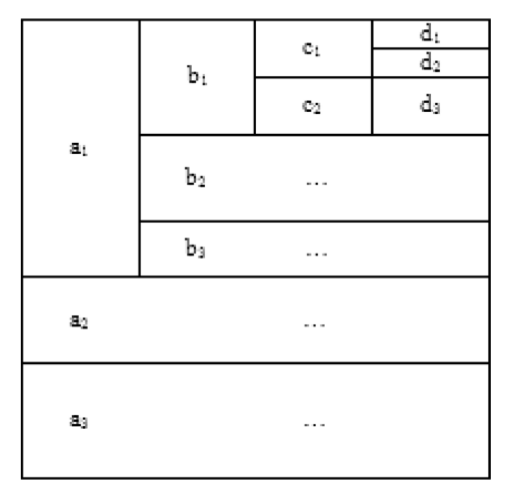
\includegraphics[width=1.7in]{picture/ch_current_research/BUC_partition} 
\caption{BUC 使用维属性的划分}\label{BUC_partition} 
\end{figure} 


\begin{figure}[!htb]
\centering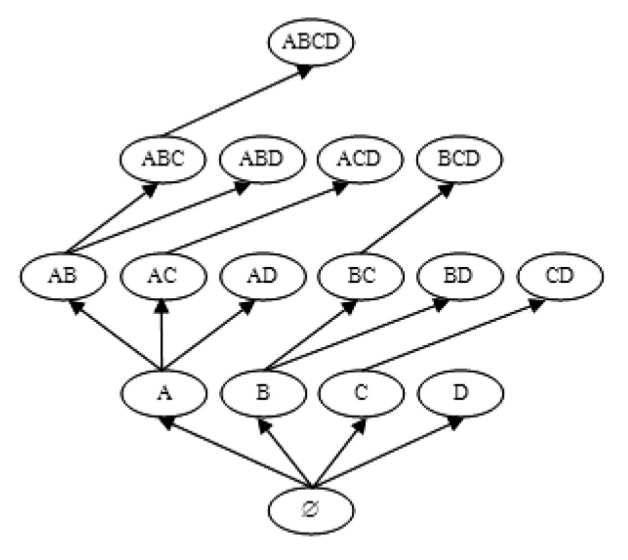
\includegraphics[width=3in]{picture/ch_current_research/BUC_execution} 
\caption{BUC 的执行过程}\label{BUC_execution} 
\end{figure} 

BUC 与 MapReduce  的结合,虽然可以利用 MapReduce 的排序以及对计算的并行处理功能,但相比之下,并不如 PiepSort 与 MapReduce 的结合,一个重要的原因是 BUC 需要对同一组数据进行多次扫描。BUC 会对数据不断地进行递归分组,它首先计算粗粒度的group,在满足阈值的条件下再继续递归计算细粒度的group。在这个过程中,同一组数据会被多次扫描,这个与reducer的迭代器仅能对数据扫描一次的功能无法很好地结合。这也正是 TSP-Cube 提出使用 PipeSort 替代 BUC 的原因。



\section{面向代数度量的分布式数据立方计算}

随着数据集大小和维度数量的增长,单机的内存和计算力已经无法满足数据立方的计算要求。因此业界开始研究利用分布式计算的优势实现数据立方的方法。\cite{nandi2011distributed} \cite{dehne2006cgmcube} \cite{ng2001iceberg} \cite{lee2012efficient}  \cite{dehne2006cgmcube}

%gmCUBE \cite{dehne2006cgmcube}、RP、BPP、ASL、PT \cite{ng2001iceberg} 这些算法都是基于由少量 PC 机组成的集群实现的,并没有与 MapReduce 框架相结合。 
%\cite{you2008parallel} \cite{sergey2009applying} \cite{lee2012efficient} 虽将数据立方的计算与 MapReduce结合,但无法很好地处理整体性度量函数的计算,也并没有考虑到数据倾斜的情况。

在这个小节中将介绍数据立方与 MapReduce 的结合,这个结合是分布式数据立方的Naive算法 \cite{nandi2011distributed}。该算法在MapReduce框架下与代数度量有非常好的整合,但与整体性度量的整合效果欠佳,因此本小节除了介绍该算法外,还会分析该算法与这两类度量函数整合效果有所差异的原因,从而引出下一节面向整体性度量的分布式数据立方计算。


\subsection{数据集}

在接下来的章节中需要数据集作为例子,因此首先介绍作为例子的数据集,这里使用\cite{nandi2011distributed}  中的数据集。数据集的表结构如图 \ref{dataset_table4} 所示。表中数据记录的是不同地区的用户的查询记录。属性id为表的主键,记录每条记录的id;time为查询时间;uid为用户的id。表中剩余的 6 个属性为维属性,分别是 country,state,city,topic,category,subcategory。其中 country,state,city 记录地区信息,topic,category,subcategory 记录查询内容。并且[country, state, city] 是具有层次型的,同理 [topic, category, subcategory] 也是具有层次性的。因此在 GroupBy 时,GroupBy(country, state, topic) 和 GroupBy(state, topic)是等价的。并且不会出现 GroupBy(country, city, topic) 这样的跨越层次的操作。

该数据集对应的 lattice 如图 \ref{dataset_lattice4} 所示。图中的 ``*" 表示不需要聚合的属性。因为数据集具有层次型,因此lattice与上一章中看到的有所不同。对于无层次型的数据集,若有 D 个维属性,则 lattice 中有${2}^{D}$ 个节点,但由于这个数据集具有层次型,因此节点数有所减少。例如对于 (country, state, city) 这3个属性的 GroupBy,仅有 3 种结果,即 GroupBy(country),GroupBy(country, state) (或 GroupBy(state)) 以及 GroupBy(country, state, city) (或 GroupBy(city))。因此该数据集对应的lattice中共有16个region,也就是该数据集共有16种 GroupBy 类型。


\begin{figure}[!htb]
\centering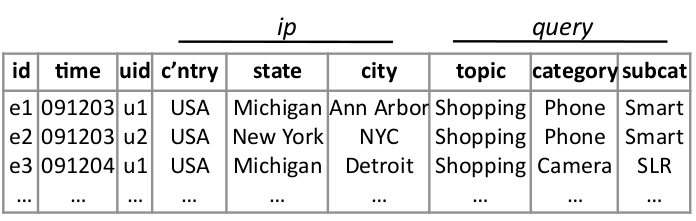
\includegraphics[width=3.2in]{picture/ch_datacube_mr/dataset_table} 
\caption{数据集的表结构}\label{dataset_table4} 
\end{figure} 

\begin{figure}[!htb]
\centering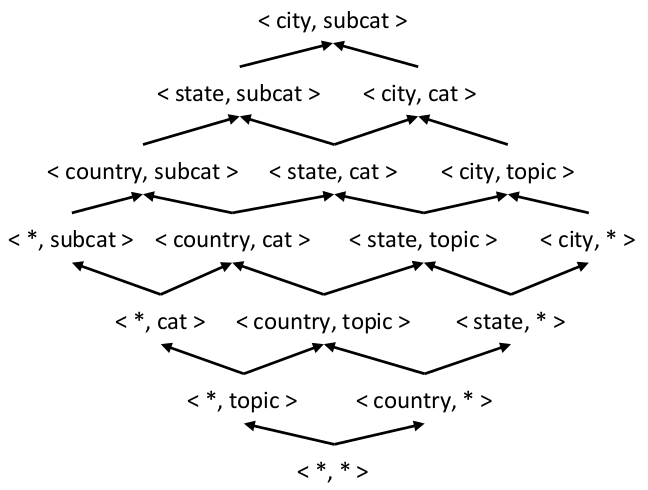
\includegraphics[width=2.7in]{picture/ch_datacube_mr/dataset_lattice} 
\caption{数据集的lattice}\label{dataset_lattice4} 
\end{figure} 

\subsection{Naive 算法实现}
 
算法 \ref{naive_algorithm} 为使用 MapReduce 计算数据立方的 Naive 实现。上述的数据集共有16个 region,那么对于输入的每一条记录,将其映射成对应的所有 group,并且与度量属性的值组成 key-value 作为 mapper 的输出。相同 key 值的数据将分派到同一个 reduce 函数中,也即相同 group 值的数据被分派到同一个 reduce 函数中,再进行聚合计算。例如输入的一条记录为 (e1, 091203, u1, USA, New Youk, NYC, Shopping, Phone, Smart),度量函数为 COUNT(DISTINCT(uid)),该度量函数是计算group内有多少不同的uid。对于这条记录,map 需要输出 16 个 ([group value], [uid]) 这样的 key-value,分别为([*,*], [u1]), ([*,Smart], [u1]), ([USA, *], [u1])等等。之后,reducer 再对同一个 group 内的数据进行聚合计算。

{\renewcommand\baselinestretch{1} 
\begin{algorithm}[!ht]
\caption{Naive Algorithm}
\label{naive_algorithm}
{\fontfamily{\familydefault}\selectfont

	\begin{algorithmic}[1] %每行显示行号
    \Function {MAP}{e}
    	\State e is a tuple in the dataset
        \ForAll {Region R in C}
        	\State k=R(e)
        	\State EMIT([k], [e])
        \EndFor
   	 \EndFunction
     \State
     \Function {REDUCE}{k,$\left\{ e1,e2,...\right\}$}
     	\State let M be measure function
        \State EMIT(k, M($\left\{ e1,e2,...\right\}$))
     \EndFunction
	\end{algorithmic}
}
\end{algorithm}
\par}

Naive的方法实现起来非常简单,对于较小的数据集也有很好的效果,但是随着数据集规模的增大,Naive方法的不足则较为明显,主要包括以下两个方面。

\begin{itemize}

\item \textbf{中间数据过多}

若 lattice 中的 region 数量为 $|C|$,数据集的大小为 $|D|$,则中间数据的数据量为 $|C|\times |D|$。随着维属性数量的增加与层次的加深,中间数据的数据量则会巨增,必然导致 map 阶段有大量的磁盘 I/O,以及 shuffle(sort) 阶段有大量的数据需要排序,对整体的效率有非常大的影响。

\item \textbf{超大group}

在 MapReduce 计算中,总体的计算时间是由计算时间最长的 reducer 决定。因此若各个 reducer 分配到的要计算的数据量差异较大时,会导致某些 reducer 运行时间远大于其他 reducer。 在 Naive 的计算方法中,具有相同 group 值的数据会在同一个 reducer 中计算,当一个 group 很大时,例如 lattice 中处于底层的 region 中的 group 相对就会较大,它运行的时间就会很长,而其他处理小 group 的 reducer 因为较早处理完数据,可能会空闲等待,甚至重新启动大 group 的计算,但重启计算效果往往不佳,最终导致整个 MapReduce 的计算时间过长。

\end{itemize}

以上两个不足,主要出现在整体性度量函数的计算中,而对于代数度量函数,例如SUM,COUNT,AVG 等,则不会有以上的问题。因为MapReduce的combiner机制与代数度量函数的计算有非常好的整合。combiner 是 MapReduce 一个重要的机制,它等同于本地的 reducer。它会对 mapper 的输出进行一次本地的 reduce 计算,然后再将数据发到相应的 reducer 上,这样可以减少网络传输的数据量和reducer 的计算量。正因为这个 combiner 的作用,对于代数度量函数,combiner 可以在本地对同一个 group 内的数据进行一次计算,将一个 mapper 上同一个 group 内的数据压缩成一条记录发送给 reducer,而不是将这个 group 内的数据直接发送到 reducer上,这样每个 reducer 获得的数据量比不使用 combiner 获得的数据量要少得多。由于mapper的数量是有限的,那么分发到一个reducer上一个group内的数据也是有限的。这样有限的数据必然不会导致中间数据过多和各个reducer上数据的不均匀。因此代数度量函数与MapReduce有较好的整合。实验部分也会对这两种度量进行比较。

但是对于整体性度量函数,combiner的作用却可能很小,这也是整体性度量函数与代数度量函数最大的区别,因为整体性度量函数中间结果的数据量是不确定的。例如对于COUNT(DISTINCT(uid))的计算,combiner可将同一个group内多条具有相同uid的记录压缩成一条输出,若uid取值较多,甚至无重复,则combiner几乎无法发挥作用。那么就会出现以上提到的两个问题。因此针对这两个问题,\cite{nandi2011distributed}提出了面向整体性度量的分布式数据立方计算方法。



\section{面向整体性度量的分布式数据立方计算}

随着数据复杂性的增加,仅使用代数度量函数并不能满足分析统计的需要。在 \cite{nandi2011distributed} 中对搜索日志的分析使用了COUNT(DISTINCT(User))、TOPK(Query)等整体性度量函数。若使用 Naive 算法直接计算这些整体性度量函数,则会出现上一节提到的中间数据过多、超大group导致负载不均衡的问题。MR-Cube \cite{nandi2011distributed} 的提出正是为了解决整体性度量函数导致的这两大类问题。

本小节将对 MR-Cube 进行具体的分析。MR-Cube针对Naive算法的不足,提出了几点改进,主要包括整体性度量的划分;使用采样的方法确定需要划分的group,减轻负载不均衡的情况;提出了Batchh Area的概念,将多个group合并在同一个reduce函数内计算,减少中间数据的产生。在分析MR-Cube贡献的同时,也对其存在的不足和可改进的地方进行分析,从而为TSP-Cube的提出提供基础。


\subsection{整体性度量的划分}

对于大 group 的问题,可以将一个大 group 划分成多个子 group,将这些子 group 分发到多个 reducer 上计算,即可解决 reducer 计算数据量不均匀的问题。

对于代数度量函数,数据是可以随意划分的。但是整体性度量函数的划分就没有这么简单了。例如整体性度量函数 COUNT(DISTINCT(uid)),它是计算不同的 uid 的数量。如果对数据集进行随意的划分,每个子块的计算结果是不同的 uid 列表,即对子块中相同的uid只保留一个。然后再对这些 uid 列表进行统计计算 COUNT(DISTINCT(uid))。这里每个子块的计算结果不能是COUNT(DISTINCT(uid)),这样会导致最终结果是错误的。中间结果是不同的 uid 列表,如果 uid 重复度非常高,那么各个列表中uid的数量较少,这种划分计算方法是可行的。但倘若 uid 的重复度非常低,各个列表的uid很可能跟子块中uid数量同样多,那么这种随意划分的方法则毫无作用。 

因此 MR-Cube 提出了一种对整体性度量函数进行划分的方法,称为部分代数度量 (Partially Algebraic Measure)。例如对于 COUNT(DISTINCT(uid)) 的度量计算,数据可按照 uid 进行划分,那么具有相同 uid 的记录会被划分到同一个子块中,而每个子块之间的 uid 是不会有相同的。这样对于每个子块都可以输出一个整数,即该子块 COUNT(DISTINCT(uid)) 的结果,最后将各个子块的结果相加即可得到最终结果。论文中将 uid 这样的用来划分的属性称之为代数属性。这样的划分方式对于很大部分的整体性度量都是有效的,例如TopK,MODE等。


\subsection{Reducer-Unfriendly Group}

确定了数据的划分方法,下一个问题是哪些 group 需要划分,也就是哪些 group 是较大的 group。在论文中使用了随机均匀采样的方式选取部分的数据进行数据立方的计算,在每个 group 内做 COUNT,也就是统计每个 group 的大小,然后根据数据集大小、采样数量、reducer limit(根据内存大小估算一个reducer可处理的数据量)以及使用切尔若夫界确定一个 group 是否是 reducer-unfriendly group。用直观的理解即是,通过概率统计的方式确定采样中的 group 是否是较大的 group,这些 group 被称为 reducer-unfriendly group。并且对于 unfriendly 的 group,会根据group的大小以及reducer limit 估算出划分因子。对于划分因子的直观理解,即是这样一个大 group 应该划分多少子块,才能令每个子块不超过 reducer 处理数据量的上限。

若一个 region 中有一个 group 是 reducer-unfriendly 的,那么这个 region 也就是 reducer-unfriendly 的。在采样后的正式计算中,对于 reducer-unfriendly region 内的所有 group 都需要进行划分。划分的方式使用上一节中提到的对整体性度量的划分方式,即根据某一个代数属性,如 uid 进行划分。如图\ref{region_partition}所示,根据采样的结果将region划分成了 friendly 和 unfriendly 两类。对于 unfriendly 的 region,region 内的所有 group 都需要划分,论文中使用取模方式进行划分。

\begin{figure}[!htb]
\centering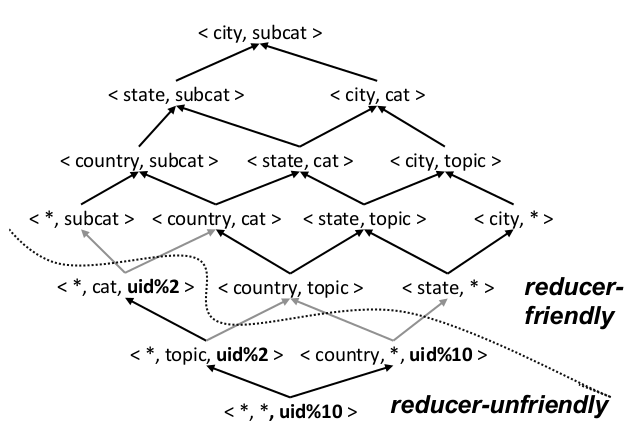
\includegraphics[width=3.5in]{picture/ch_datacube_mr/region_partition} 
\caption{根据uid被划分的lattice}\label{region_partition} 
\end{figure} 

上述的方法只记录需要划分的region,这是因为 region 的数量远比 group 少得多。若要记录所有的需要划分的 group,则需要太大的开销。只记录region的方法能保证大 group 的划分,但是如果 region 中只有 1 个 group 是 unfriendly 的,其他的friendly 的 小group 也要被迫划分,这样将导致不必要的划分以及出现过多的被划分数据,加重了最后的合并操作。同时,论文中使用了取模的方式进行划分,这样的哈希方式非常简单,在很多情况下也是有效的,但是在一些情况下,很可能导致划分的不均匀。就这两点不足,MR-Cube的划分方式仍有可改进的空间。

\subsection{Batch Area}

对于Naive方法中的另一个问题,中间数据过多的问题,MR-Cube中提出了 Batch Area 的概念。也就是利用 region 之间的父子关系,将多个 group 放在同一个 reduce 函数中计算,而不是像 Naive 的方法,一个 reduce 函数只计算一个 group。论文中给出了划分 batch 的一些规则,规则包括以下几点。
\begin{itemize}
\item reducer-unfriendly 的 region 和 reducer-friendly 的 region 不可划分在同一个batch内。
\item 对于 reducer-unfriendly region 的划分,同一个 batch 内的 region 需要有相同的划分因子。
\item 同一个 batch 中的 region 需要有父子关系。
\item 两个 batch 的 region 数量差别不能超过2。
\end{itemize}

图\ref{batch_area}是其中一种合乎规则的划分方式。图中使用虚线将各个batch加以划分。

\begin{figure}[!ht] 
\centering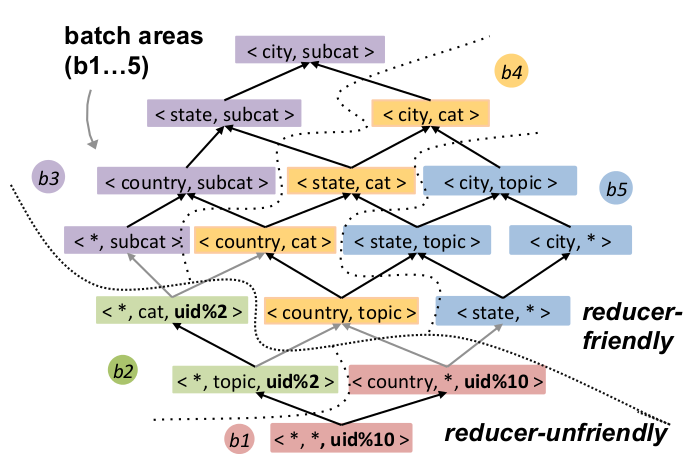
\includegraphics[width=3.5in]{picture/ch_datacube_mr/batch_area} 
\caption{Batch Area}\label{batch_area} 
\end{figure}

对于同一个 batch 内的 group 要如何计算有很多方法,论文使用的是BUC(BottomUpCube)。但这种方法需要对同一组数据扫描多次,而 Mapreduce 的 reducer 中提供的迭代器仅能对数据扫描一次,若要对数据进行多次扫描,则需要先载入内存,这样将导致过多的内存开销。对于BUC的具体实现,将在下一节中详细阐述,并分析其与MapReduce的结合、与PipeSort的比较。同时,论文中只给出了batch 划分的规则,提到可用枚举、局部贪心或者模拟退火的方式找出合乎规则的划分,并没有给出具体的方法,而模拟退火这样的计算方法又稍微复杂。因此这里可以考虑提出简单而有效的划分方法。


\subsection{贡献与不足}

MR-Cube \cite{nandi2011distributed} 这篇论文对使用 Naive 算法计算整体性度量函数的数据立方中存在的问题提出了一些非常有效的改善方法,论文的主要贡献包括:

\begin{enumerate}
\item 提出了对整体性度量划分的方法。
\item 提出了如何判断 group 是否需要划分,以及其划分的方法。
\item 提出了将多个 group 合并计算的 batch area 的概念。
\end{enumerate}

但是以上的方法也存在一些问题。

\begin{enumerate}
\item 论文中通过 region 内的一个大 group 将一个 region 内的所有 group 都贴上 reducer-unfriendly 的标签,导致 region 内所有的 group 都要划分。有些情况下可能一个 region 就只有一个大 group,而其他的 group 都很小,这样就导致了不必要的划分和加重后续的合并操作。
\item 论文中使用取模(\%)方法对数据进行划分,取模是一种简单有效的哈希方法,但是这种哈希方法在一些情况下,可能会导致划分的不均匀。
\item Batch area 的计算,也就是多个 group 之间的计算,论文里使用了 BUC 的方法,虽然这种方法很合适有阈值限定的情况(例如 HAVING),但是它需要对同一组数据进行多次扫描,而MapReduce中reducer的迭代器仅能对数据扫描一次,若要多次扫描则需将数据载入内存或者读写文件,这将导致过多的内存和I/O开销。
\item 论文中只给出了 batch area 的规则,并没有提供简单且能满足规则的划分方法。
\end{enumerate}

针对以上4点,本论文提出了 TSP-Cube 算法, 尝试改进 MR-Cube 的不足。


